\documentclass[a4paper,11pt]{article}
\usepackage[utf8]{inputenc}
\usepackage{minted}
\usepackage{amsmath}
\usepackage{float}
\usepackage{graphicx}
\usepackage[toc,page]{appendix}

\graphicspath{{./figures/}}

\title{\textbf{9. Priority queue}}
\author{Kristiāns Vinters}
\date{Fall 2023}

\begin{document}
    \maketitle
    \section*{Introduction}

    I solved the assignment in Go. I used Go because I want to become more familiar with it. Source code and benchmark data is available on GitHub\footnote{https://github.com/Phanty133/id1021/tree/master/9-heap}.

    \section*{Implementation}

    Implementing the two linked list versions was simple, however getting the heap versions working was a bit more tricky because it was easy to make a trivial mistake that was hard to spot. I implemented all of the priority queues to fit a common interface to make benchmarking more straightforward.

    \begin{minted}{go}
type PriorityQueue[T comparable] interface {
    Add(val T, priority int)
    Remove() (T, error)
    Empty() bool
}
    \end{minted}

    The linked list priority queue implementations only differ in the implementations of their add and remove functions. The base data type is the same and basically just a wrapper around a linked list. The linked list implementation is reused from a previous assignment. The linked list priority queues are implemented in such a way that a higher priority value will get removed first, unlike the other implementations which are min-heaps.

    \begin{minted}{go}
type PQueueLLFastAdd[T comparable] struct {
    list *llist.LinkedList[PriorityQueueItem[T]]
}

type PQueueLLFastRemove[T comparable] struct {
    list *llist.LinkedList[PriorityQueueItem[T]]
}

type PriorityQueueItem[T comparable] struct {
    Value    T
    Priority int
}
    \end{minted}

    The \texttt{PQueueLLFastAdd} implementation adds new elements to the start of the list, which is an $O(1)$ operation, and finds the next node to remove with a linear search, which is an $O(n)$ operation.
    
    \begin{minted}{go}
func (h *PQueueLLFastAdd[T]) Remove() (T, error) {
    if h.Empty() {
        var zero T
        return zero, errors.New("heap empty")
    }

    var min *llist.LinkedListItem[PriorityQueueItem[T]]
    min = nil

    // Keep track of prev nodes to make node removal O(1)
    var minPrevNode *llist.LinkedListItem[PriorityQueueItem[T]]
    var prevNode *llist.LinkedListItem[PriorityQueueItem[T]]
    minPrevNode = nil
    prevNode = nil

    // Iterate to find the next highest priority node
    for node := range h.list.Iter() {
        if min == nil || min.Head.Priority < node.Head.Priority {
            min = node
            minPrevNode = prevNode
        }

        prevNode = node
    }

    // Remove the node from the list
    if minPrevNode == nil {
        h.list.SetFirst(min.Next())
    } else {
        minPrevNode.SetNext(min.Next())
    }

    return min.Head.Value, nil
}        
    \end{minted}

    The \texttt{PQueueLLFastRemove} functions are reversed - with \texttt{Remove()} it removes the first node, and with \texttt{Add()} it finds the correct place to insert the new node with a linear search. The implementation for the linear search function is almost the same as for the \texttt{PQueueLLFastAdd.Remove()}, so I won't include it here.

    For the linked heap-based priority queue, the main structure was still simple and largely just wrapped the root node, while the node structure became more complex compared to a linked list node structure.

    \begin{minted}{go}
type Heap[T any] struct {
    root *HeapNode[T]
}

type HeapNode[T any] struct {
    size     int
    priority int
    Value    T
    left     *HeapNode[T]
    right    *HeapNode[T]
}
    \end{minted}

    I implemented the \texttt{Add} and \texttt{Remove} functions recursively.

    \begin{minted}{go}
func (h *Heap[T]) Add(val T, priority int) {
    // If the heap is empty, create a new root node
    if h.root == nil {
        h.root = newHeapNode[T](val, priority)
        return
    }

    // Recursively travel the heap to find the correct place
    // to insert the new node
    h.root.Add(val, priority)
}

func (h *HeapNode[T]) Add(val T, priority int) {
    h.size++

    // If the new node has a higher priority than the current
    // node, swap them
    if priority < h.Priority() {
        h.Value, val = val, h.Value
        h.priority, priority = priority, h.priority
    }

    // If the current node has no children, create new children
    if h.left == nil {
        h.left = newHeapNode[T](val, priority)
        return
    }

    if h.right == nil {
        h.right = newHeapNode[T](val, priority)
        return
    }

    // If the left subtree is smaller than the right subtree, add
    // the new node to the left subtree
    if h.left.Size() <= h.right.Size() {
        h.left.Add(val, priority)
        return
    }
    
    // Otherwise, add the new node to the right subtree
    h.right.Add(val, priority)
}
    \end{minted}

    The \texttt{Heap.Remove()} function has a very similar structure to the \texttt{Heap.Add()} function, as it also initiates a recursive chain, however, the \texttt{HeapNode.Remove()} function differs.

    \begin{minted}{go}
func (h *HeapNode[T]) Remove() {
    h.size--

    var promoted *HeapNode[T]

    // Promote the node with the highest priority
    // or if only one exists, the only node.
    if h.left == nil {
        promoted = h.right
    } else if h.right == nil {
        promoted = h.left
    } else if h.right.Priority() < h.left.Priority() {
        promoted = h.right
    } else {
        promoted = h.left
    }

    // Swap values with the promoted node
    h.Value = promoted.Value
    h.priority = promoted.priority

    // If the promoted node has no children,
    // remove the node and end the recursion
    if promoted.size == 0 {
        if promoted == h.left {
            h.left = nil
        } else {
            h.right = nil
        }
    } else {
        promoted.Remove()
    }
}
    \end{minted}

    I implemented the \texttt{HeapNode.Push()} function with a loop instead of recursion to make tracking the depth simpler. The logic is similar to the \texttt{HeapNode.Remove()} function.

    \begin{minted}{go}
func (h *HeapNode[T]) Push(incr int) int {
    h.priority += incr
    depth := 0

    curNode := h
    var nextNode *HeapNode[T] = nil

    // Loop until we reach a leaf node
    for curNode != nil {
        // Determine the next node with the highest priority
        if curNode.left == nil {
            nextNode = curNode.right
        } else if curNode.right == nil {
            nextNode = curNode.left
        } else if curNode.left.Priority() < curNode.right.Priority() {
            nextNode = curNode.left
        } else {
            nextNode = curNode.right
        }

        // If there was no next node determined or if the highest priority node
        // still has a lower priority than the current node, terminate the loop
        if nextNode == nil || nextNode.Priority() > curNode.Priority() {
            break
        }

        // Swap values and priorities
        curNode.Value, nextNode.Value = nextNode.Value, curNode.Value
        curNode.priority, nextNode.priority = nextNode.priority, curNode.priority
        depth++

        // Move to the next node
        curNode = nextNode
    }

    return depth
}
    \end{minted}

    The array-based heap had a simpler implementation. I used a slice to store the heap, to avoid having to deal with resizing the array. The \texttt{Add()} and \texttt{bubble()} functions were straightforward to implement:
    \begin{minted}{go}
func (h *ArrHeap[T]) Add(val T, priority int) {
    newNode := ArrHeapNode[T]{Value: val, priority: priority}
    h.data = append(h.data, newNode)
    h.bubble()
}

func (h *ArrHeap[T]) bubble() {
    n := len(h.data) - 1

    for n > 0 {
        var parent int

        // Calculate the parent node
        if n%2 == 0 {
            parent = (n - 2) / 2
        } else {
            parent = (n - 1) / 2
        }

        if h.data[parent].priority <= h.data[n].priority {
            break
        }

        h.data[parent], h.data[n] = h.data[n], h.data[parent]
        n = parent
    }
}
    \end{minted}

    The \texttt{Remove()} and \texttt{sink()} functions had equally straightforward logic, however the \texttt{sink()} had to cover more cases like checking for empty branches, so it resulted in appearing more complex.

    \section*{Benchmarking}

    I ran 3 different benchmarks - adding N elements, removing N elements from a preprepared queue, and comparing \texttt{Push()} vs \texttt{Add()/Remove()}. I ran the first two benchmarks on all four implementations, and the third benchmark only on the linked heap implementation. I ran the benchmarks on my laptop with an AMD Ryzen 5600H and 16GB of RAM using Go v1.21.3. The Go code generated \texttt{.csv} files, which were then analyzed in LibreOffice Calc.

    \subsection*{Adding N elements}

    I ran the benchmark with N ranging from 100 to 50000 for linked list-based priority queues, but from 100 to 1000000 for the heap-based priority queues. The results are shown in Figure \ref{fig:add}.

    \begin{figure}[H]
        \centering
        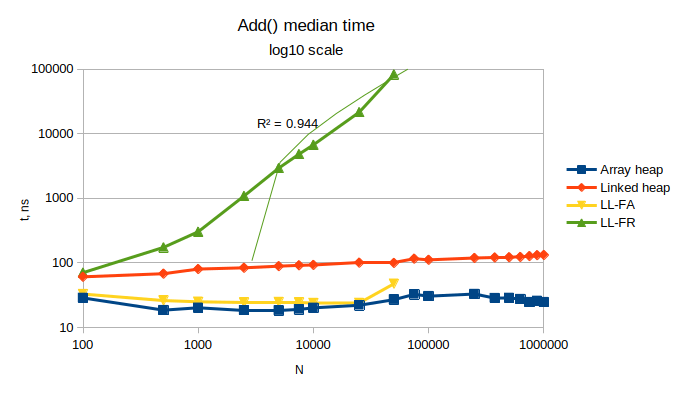
\includegraphics[width=\textwidth]{add.png}
        \caption{Median enqueue times. LL-FA = Linked list fast add, LL-FR = Linked list fast remove}
        \label{fig:add}
    \end{figure}

    As expected, the linked list-based priority queue that removes elements by searching for the next highest priority has an approximately $O(n)$ complexity, whereas both heap implementations and the linked list queue that just adds elements at the start of the list have an approximately $O(1)$ complexity. The fastest implementation in this benchmark is the fast add linked list, as it doesn't need to perform any other action with the node apart from adding it, whereas the heaps need to bubble nodes. The difference between the coefficients between the array heap and linked heap can be explained by the linked heap having to allocate new nodes with every addition, whereas the array heap can allocate a larger chunk of memory at once, thus reducing overhead.

    \subsection*{Removing N elements}

    I ran the benchmark with N ranging from 100 to 50000 for linked list-based priority queues, but from 100 to 1000000 for the heap-based priority queues. The results are shown in Figure \ref{fig:remove}.

    \begin{figure}[H]
        \centering
        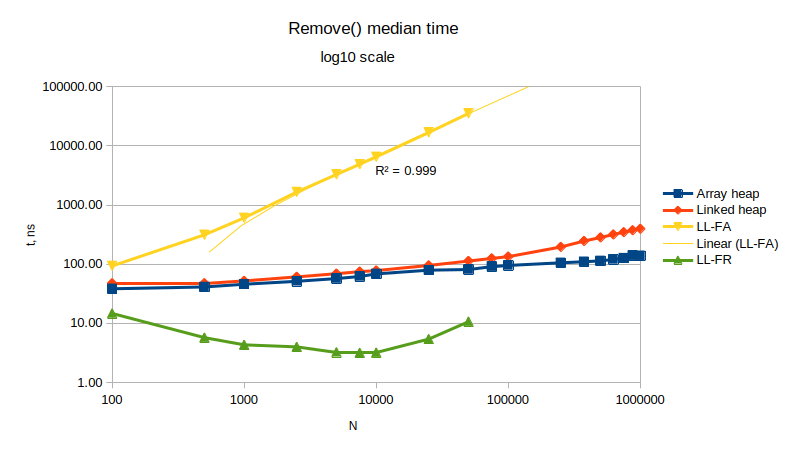
\includegraphics[width=\textwidth]{remove.png}
        \caption{Median Dequeue times. LL-FA = Linked list fast add, LL-FR = Linked list fast remove}
        \label{fig:remove}
    \end{figure}

    As in the previous benchmark, the non-optimized linked list queue, LL-FA in this case, has a linear complexity because it needs to perform a linear search for the next highest priority node. The fast remove times appear to be noisy, so estimating a complexity is difficult, but it appears to be closer to $O(1)$. Which is to be expected because the $Remove()$ function only needs to remove the first node, which is guaranteed to be the next highest priority by the $Add()$ function. The heap implementations are expected to have a complexity of $O(log_2{(n)})$. They appear to trend upward at a significantly lesser rate compared to the $O(n)$ function, however, they don't perfectly correlate when graphed against $log_2{(n)}$ (Fig. \ref{fig:complexity})

    \begin{figure}[H]
        \centering
        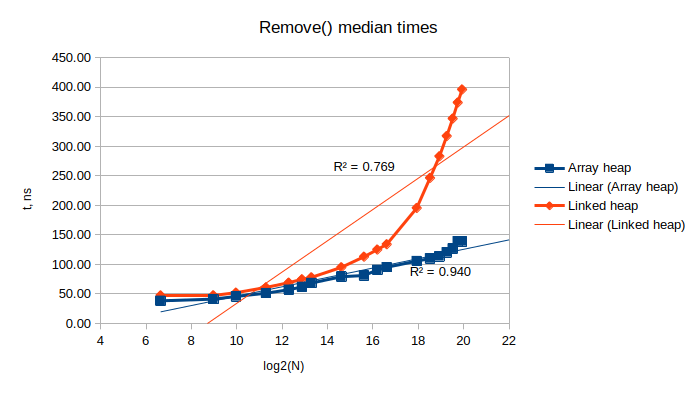
\includegraphics[width=\textwidth]{complexity.png}
        \caption{Heap median dequeue times vs $log_2{(n)}$}
        \label{fig:complexity}
    \end{figure}

    The array heap implementation appears to have a decent fit at $R^2=0.940$, whereas the linked heap appears to have a significantly worse fit at $R^2=0.761$ as a result of an unexpected increase in execution time at larger $N$. It's possible that it's an issue with the implementation, however, I couldn't find any obvious issues. Another possibility is that it's because the nodes need to be deallocated after removal, which could be a bottleneck at larger $N$, compared to the array heap, which would get reduced in size only occassionally and in larger chunks.

    In the case of preferring one linked list queue implementation over the other, it might make sense to use a fast add implementation for a queue that needs to handle a large influx of elements, but doesn't need to remove elements as fast. A possible real-world usecase might be a queue for handling network requests. We would want to acknowledge that a request has been received as quickly as possible, but we might not need to process it immediately. A possible use-case for a fast-remove linked list priority queue might be a queue for handling tasks that need to be processed as quickly as possible, but we don't need to add tasks to the queue as quickly, for instance, a slowly accumulating job/dataset pool, which gets processed in batches.

    \subsection*{Push() vs Add()/Remove()}

    To compare the \texttt{Push()} and \texttt{Add()/Remove()} functions, I generated a random queue of N elements, then incremented the root element priority 500 times by a random number from 1 to 10000. I ran the benchmark with N ranging from 100 to 100000. The results are shown in Figure \ref{fig:push}.

    \begin{figure}[H]
        \centering
        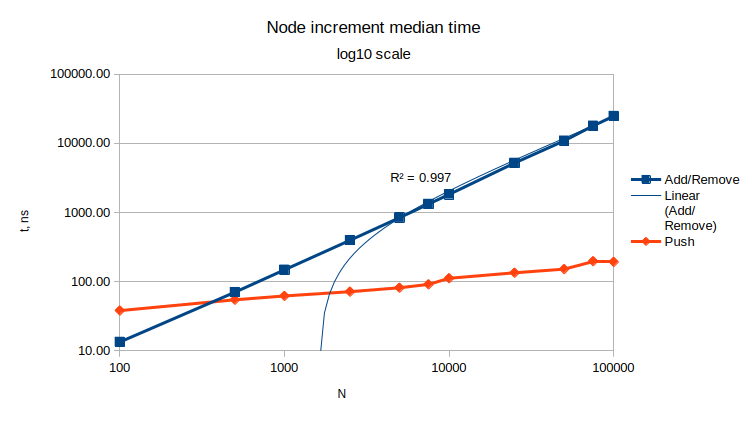
\includegraphics[width=\textwidth]{push.png}
        \caption{Median priority increment times}
        \label{fig:push}
    \end{figure}

    At $N=100$, the \texttt{Add()/Remove()} approach appears to perform better than \texttt{Push()}, getting a median 13ns per increment vs a median 38ns. However, at higher $N$, the \texttt{Push()} approach performs significantly better. \texttt{Add()/Remove()} fits a complexity of $O(N)$, whereas \texttt{Push()} times strongly correlate ($R^2=0.888$) with a complexity of $O(log_2({n}))$ (fig. \ref{fig:push-complexity}), which is what is expected for a binary heap.

    \begin{figure}[H]
        \centering
        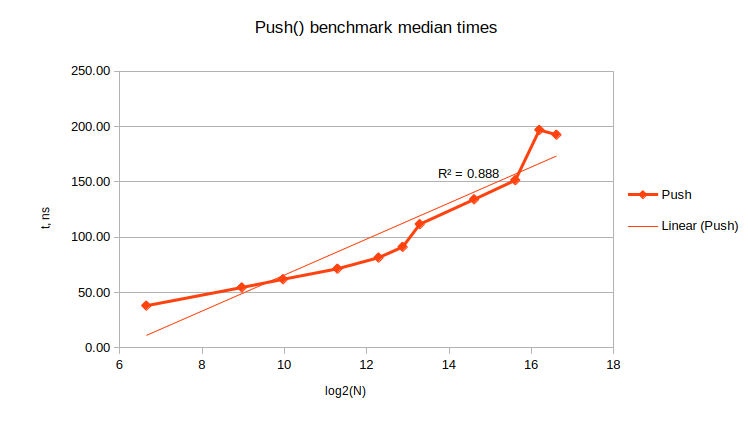
\includegraphics[width=\textwidth]{complexity-push.png}
        \caption{\texttt{Push()} median execution times graphed vs $log_2{(n)}$}
        \label{fig:push-complexity}
    \end{figure}

    \subsubsection*{Push() depth}

    I measured the mean depth a $Push()$ operation would have to travel when incrementing a node. I ran the benchmark with queue sizes ranging from 100 to 100000. The results are shown in Figure \ref{fig:push-depth}.

    \begin{figure}[H]
        \centering
        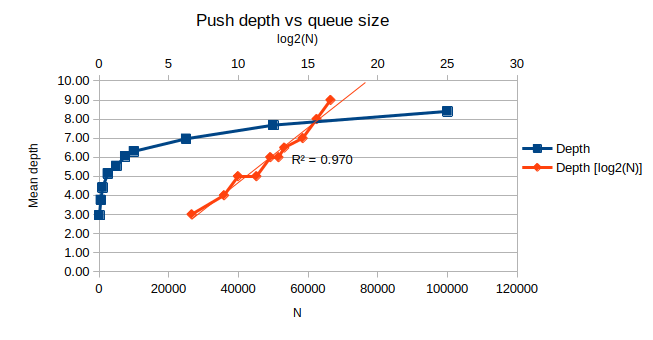
\includegraphics[width=\textwidth]{depth.png}
        \caption{Mean depth of a \texttt{Push()} operation. Depth is plotted both against a linear queue size and a logarithmic queue size.}
        \label{fig:push-depth}
    \end{figure}

    The mean travel depth of a \texttt{Push()} operation appears to strongly correlate with a $log_2({n})$ function ($R^2=0.970$). For all queue sizes, the minimum travel depth was 0, in the case that the increment wasn't enough to make the root node not the highest priority node. The theoretical maximum depth is $\lfloor \log_2{(n)}\rfloor + 1$, however, none of my benchmarks at any size reached that depth (fig. \ref{fig:depth-table}).

    \begin{figure}[H]
        \centering
        \begin{tabular}{c|c|c|c|c}
            N & Mean depth & Actual max reached & Theoretical max depth & $\frac{\text{Actual}}{\text{Theoretical}}$ \\
            \hline
            \hline
            100 & 2.96 & 5 & 7 & 0.71 \\
            500 & 3.76 & 7 & 9 & 0.78 \\
            1000 & 4.41 & 7 & 10 & 0.70 \\
            2500 & 5.14 & 8 & 12 & 0.67 \\
            5000 & 5.54 & 8 & 13 & 0.62 \\
            7500 & 6.05 & 9 & 13 & 0.69 \\
            10000 & 6.31 & 10 & 14 & 0.71 \\
            25000 & 6.97 & 10 & 15 & 0.67 \\
            50000 & 7.68 & 11 & 16 & 0.69 \\
            100000 & 8.41 & 12 & 17 & 0.71 \\
        \end{tabular}
        \caption{Theoretical max depth vs max depth reached}
        \label{fig:depth-table}
    \end{figure}
\end{document}
